\documentclass[tikz,border=5pt,10pt]{standalone}
% Shared style for the auditor figures, following the TSE/ALIGN papers: steps are rounded
% blue boxes, data are slanted yellow boxes, stores are purple cylinders, model calls orange.
\usepackage[T1]{fontenc}
\usepackage{lmodern}
\usepackage[scaled=0.92]{helvet}
\renewcommand{\familydefault}{\sfdefault}
\usepackage{fontawesome5}
\hyphenpenalty=10000\exhyphenpenalty=10000
\usetikzlibrary{positioning,arrows.meta,calc,fit,backgrounds,shapes.geometric}
\definecolor{pBlue}{HTML}{DAE8FC}\definecolor{pBlueD}{HTML}{6C8EBF}
\definecolor{pGreen}{HTML}{D5E8D4}\definecolor{pGreenD}{HTML}{82B366}
\definecolor{pOrange}{HTML}{FFE6CC}\definecolor{pOrangeD}{HTML}{D79B00}
\definecolor{pYellow}{HTML}{FFF2CC}\definecolor{pYellowD}{HTML}{D6B656}
\definecolor{pRed}{HTML}{F8CECC}\definecolor{pRedD}{HTML}{B85450}
\definecolor{pPurple}{HTML}{E1D5E7}\definecolor{pPurpleD}{HTML}{9673A6}
\definecolor{pGrey}{HTML}{F5F5F5}\definecolor{pGreyD}{HTML}{666666}
% \ic{icon}{title}{subtitle}: a step's text, icon before the title, subtitle in grey.
\newcommand{\ic}[3]{{\color{black!65}#1}\,\textbf{#2}\\[-0.2ex]{\scriptsize\color{black!70}#3}}
\newcommand{\sub}[1]{\\[-0.2ex]{\scriptsize\color{black!70}#1}}
\newcommand{\f}[1]{\texttt{#1}}
\tikzset{
  every node/.append style={execute at begin node=\setlength{\baselineskip}{1.0em}},
  act/.style={draw=pBlueD, fill=pBlue, rounded corners=3pt, line width=0.6pt, align=center,
    minimum height=9mm, inner sep=2pt, text width=#1},
  act/.default=2.4cm,
  llm/.style={act=#1, draw=pOrangeD, fill=pOrange},
  llm/.default=2.4cm,
  rule/.style={act=#1, draw=pGreenD, fill=pGreen},
  rule/.default=2.4cm,
  dat/.style={draw=pYellowD, fill=pYellow, trapezium, trapezium left angle=75,
    trapezium right angle=105, trapezium stretches=true, align=center, minimum height=9mm,
    inner sep=1pt, text width=#1},
  dat/.default=2.5cm,
  sto/.style={draw=pPurpleD, fill=pPurple, cylinder, shape border rotate=90, aspect=0.2,
    align=center, minimum height=9.5mm, inner sep=1pt, text width=#1},
  sto/.default=2.2cm,
  out/.style={act=#1, draw=pRedD, fill=pRed},
  out/.default=2.4cm,
  grp/.style={draw=#1, dashed, rounded corners=4pt, line width=0.5pt, inner sep=1.6mm},
  ar/.style={-{Latex[length=1.6mm]}, line width=0.6pt, black!65},
  st/.style={black!55, densely dotted, line width=0.7pt},
  lab/.style={font=\sffamily\scriptsize, text=black!75, inner sep=1.5pt},
  gl/.style={font=\sffamily\scriptsize\bfseries, text=#1, inner sep=1pt},
}

% Math checker (figure*): triage picks the claims, a deep check reads each with the whole
% paper and may test it in the sandbox, a review call drops refuted findings. Labels follow
% planner/theory.py (triage_tasks), agents/theory/__init__.py, agents/theory/review.py,
% infra/sandbox.py and docker/math/Dockerfile.
\begin{document}
\begin{tikzpicture}[x=1cm, y=1cm, font=\sffamily\footnotesize]
\node[dat=2.6cm] (pp) at (0,0) {\f{ParsedPaper}\sub{every sentence with its id;\\sent once, then cached}};
\node[llm=2.8cm] (tri) at (3.35,0) {\ic{\faRobot}{Triage}{review model, medium thinking;\\two independent looks}};
\node[dat=2.9cm] (tc) at (6.85,0) {\f{TheoryClaim}s\sub{reason, kind, sentence ids,\\what it depends on; 4 per look}};
\node[llm=2.9cm] (deep) at (10.4,0) {\ic{\faRobot}{Deep check}{one claim, the whole paper\\as a cached prefix}};
\node[dat=3.0cm] (dc) at (14.0,0) {\f{DeepCheck}\sub{has error, quote, explanation,\\witness, confidence, test code}};
\draw[ar] (pp) -- (tri);
\draw[ar] (tri) -- (tc);
\draw[ar] (tc) -- (deep);
\draw[ar] (deep) -- (dc);

% the sandbox round
\node[act=3.0cm] (box) at (10.4,-1.85) {\ic{\faDocker}{Math sandbox}{SymPy, NumPy, mpmath,\\NetworkX, z3; no network, 20\,s}};
\draw[ar] ($(dc.south)+(-0.6,0)$) |- node[lab, below, pos=0.75] {test code} (box.east);
\draw[ar] ($(box.north)+(-0.5,0)$) -- node[lab, left, align=right] {output; a\\second answer} ($(deep.south)+(-0.5,0)$);

% the review, right to left
\def\yr{-3.55}
\node[out=2.6cm] (f) at (14.0,\yr) {\textbf{math error}\sub{quoted sentence,\\explanation, witness}};
\node[llm=2.9cm] (rev) at (10.4,\yr) {\ic{\faRobot}{Review}{all of the paper's findings,\\with the whole paper}};
\node[out=2.6cm] (kept) at (6.85,\yr) {\textbf{kept}\sub{to verify and rank}};
\node[act=2.3cm, draw=pGreyD, fill=pGrey] (drop) at (3.35,-3.0) {\textbf{dropped}\sub{not an error}};
\node[act=2.3cm, draw=pGreyD, fill=pGrey] (dup) at (3.35,-4.1) {\textbf{marked repeat}\sub{same as another}};
\draw[ar] ($(dc.south)+(0.6,0)$) -- node[lab, right] {error found} ($(f.north)+(0.6,0)$);
\draw[ar] (f) -- (rev);
\draw[ar] (rev) -- node[lab, above] {error} (kept);
\draw[ar] (rev.south) -- ++(0,-0.35) -| ($(dup.south)+(0.6,0)$) node[lab, pos=0.2, below] {same as};
\draw[ar] (rev.north) -- ++(0,0.3) -| ($(drop.north)+(0.6,0)$) node[lab, pos=0.2, above] {not an error};

\node[lab, anchor=north west, text width=4.6cm] at (-1.4,-1.1) {Claims the triage did not pick can get a
  cheap screen on the main model first. A paper gets at most two attempts, 30 minutes and 40 model calls.};
\end{tikzpicture}
\end{document}
